% Options for packages loaded elsewhere
\PassOptionsToPackage{unicode}{hyperref}
\PassOptionsToPackage{hyphens}{url}
%
\documentclass[
]{article}
\usepackage{amsmath,amssymb}
\usepackage{lmodern}
\usepackage{iftex}
\ifPDFTeX
  \usepackage[T1]{fontenc}
  \usepackage[utf8]{inputenc}
  \usepackage{textcomp} % provide euro and other symbols
\else % if luatex or xetex
  \usepackage{unicode-math}
  \defaultfontfeatures{Scale=MatchLowercase}
  \defaultfontfeatures[\rmfamily]{Ligatures=TeX,Scale=1}
\fi
% Use upquote if available, for straight quotes in verbatim environments
\IfFileExists{upquote.sty}{\usepackage{upquote}}{}
\IfFileExists{microtype.sty}{% use microtype if available
  \usepackage[]{microtype}
  \UseMicrotypeSet[protrusion]{basicmath} % disable protrusion for tt fonts
}{}
\makeatletter
\@ifundefined{KOMAClassName}{% if non-KOMA class
  \IfFileExists{parskip.sty}{%
    \usepackage{parskip}
  }{% else
    \setlength{\parindent}{0pt}
    \setlength{\parskip}{6pt plus 2pt minus 1pt}}
}{% if KOMA class
  \KOMAoptions{parskip=half}}
\makeatother
\usepackage{xcolor}
\usepackage[margin=1in]{geometry}
\usepackage{graphicx}
\makeatletter
\def\maxwidth{\ifdim\Gin@nat@width>\linewidth\linewidth\else\Gin@nat@width\fi}
\def\maxheight{\ifdim\Gin@nat@height>\textheight\textheight\else\Gin@nat@height\fi}
\makeatother
% Scale images if necessary, so that they will not overflow the page
% margins by default, and it is still possible to overwrite the defaults
% using explicit options in \includegraphics[width, height, ...]{}
\setkeys{Gin}{width=\maxwidth,height=\maxheight,keepaspectratio}
% Set default figure placement to htbp
\makeatletter
\def\fps@figure{htbp}
\makeatother
\setlength{\emergencystretch}{3em} % prevent overfull lines
\providecommand{\tightlist}{%
  \setlength{\itemsep}{0pt}\setlength{\parskip}{0pt}}
\setcounter{secnumdepth}{5}
\usepackage{booktabs}
\usepackage{longtable}
\usepackage{array}
\usepackage{multirow}
\usepackage{wrapfig}
\usepackage{float}
\usepackage{colortbl}
\usepackage{pdflscape}
\usepackage{tabu}
\usepackage{threeparttable}
\usepackage{threeparttablex}
\usepackage[normalem]{ulem}
\usepackage{makecell}
\usepackage{xcolor}
\ifLuaTeX
  \usepackage{selnolig}  % disable illegal ligatures
\fi
\usepackage[]{natbib}
\bibliographystyle{plainnat}
\IfFileExists{bookmark.sty}{\usepackage{bookmark}}{\usepackage{hyperref}}
\IfFileExists{xurl.sty}{\usepackage{xurl}}{} % add URL line breaks if available
\urlstyle{same} % disable monospaced font for URLs
\hypersetup{
  pdftitle={Hebbian learning can explain rhythmic entrainment to statistical regularities},
  pdfkeywords={Keywords},
  hidelinks,
  pdfcreator={LaTeX via pandoc}}

\title{Hebbian learning can explain rhythmic entrainment to statistical
regularities}
\author{Ansgar D. Endress, City, University of London\\
Ana Fló, Cognitive Neuroimaging Unit, CNRS ERL 9003, INSERM U992, CEA,
Université Paris-Saclay, NeuroSpin Center, Gif/Yvette, France}
\date{}

\begin{document}
\maketitle
\begin{abstract}
THIS IS THE ABSTRACT FROM SOME OLD PAPER. IGNORE In many domains,
organisms need to split continuous signals into sequences of recurring
units. For example, during language acquisition, humans need to split
fluent speech into its underlying words. One prominent candidate
mechanism involves computation of co-occurrence statistics such
Transitional Probabilities (TPs). TPs indicate how predictive items are
of each other. For example, items such as syllables are more predictive
of each other when they are part of the same unit (i.e., word) than when
they come from different units. TP computations are surprisingly
flexible and sophisticated. Humans are sensitive to (1) forward and
backward TPs, (2) TPs between adjacent items and longer-distance TPs and
(3) recognize TPs in both known and novel units. Here, we show that a
simple and biologically plausible model explains these data. We present
a network where excitatory interactions are tuned by Hebbian learning
and where inhibitory interactions control the overall level of
activation. We show that (1) if forgetting is weak, activations are so
long-lasting that indiscriminate associations occur among \emph{all}
items; (2) if forgetting is strong, activations are so short-lived that
they do not persist after the offset of stimuli, and no associations are
formed; and (3) for intermediate forgetting rates, this simple network
accounts for all of the hallmarks mentioned above. Ironically,
forgetting seems to be a key ingredient that enables these sophisticated
learning abilities.
\end{abstract}

\hypertarget{introduction}{%
\section{Introduction}\label{introduction}}

During language acquisition, word learning is challenging even when the
phonological form of words is known \citep{Gillette1999, Medina2011}.
However, speech in unknown languages often appears as a continuous
signal with few cues to word onsets and offsets (but see
\citep{Brentari2011, Christophe2001, Endress-cross-seg, Johnson2001a, Johnson2009, Pilon1981, Shukla2007, Shukla2011}).
As a result, learners first need to discover where words start and where
they end before than can commit any phonological word form to memory
\citep{Aslin1998, Saffran-Science, Saffran1996b} (and hopefully link it
to some meaning). This challenge is called the segmentation problem.

Learners might solve the segmentation problem using co-occurrence
statistics tracking the predictability of syllables. For example, a
syllable following ``the'' is much harder to predict than a syllable
following ``whis''. After all, ``the'' can precede any noun, but there
are very few words starting with ``whis'' (e.g., whiskey, whisker,
\ldots). The most prominent version of such co-occurrence statistics
involves Transitional Probabilities (TPs), i.e., the conditional
probability of a syllable \(\sigma_2\) following another syllable
\(\sigma_1\) \(P(\sigma_2|\sigma_1)\). In fact, infants, newborns and
non-human animals are all sensitive to TPs
\citep{Aslin1998, Chen2015, Creel2004, Endress-tone-tps, Endress-Action-Axc, Fiser2002a, Fiser2005, Flo2022, Glicksohn2011, Hauser2001, Kirkham2002, Saffran1996b, Saffran-Science, Saffran1999, Saffran2001, Sohail2016, Toro2005-backward, Turk-Browne2005, Turk-Browne-reversal}.

Following \citep{Aslin1998, Saffran-Science, Saffran1996b}, participants
in a typical behavioral Statistical Learning experiment are first
familiarized with a statistically structured speech stream (or a
sequence in another modality). The speech stream is a random
concatenation of triplets of non-sense syllables (hereafter ``words'').
For example, if \emph{ABC}, \emph{DEF}, \emph{GHJ} and \emph{KLM} are
``words'' (where each letter represents a syllable), syllables within
words are more predictive of one another than syllable across
word-boundaries. After all, the \emph{C} at the end of \emph{ABC} can be
followed by the word-initial syllables of any of the other words. A
sensitivity to TPs is then tested by measuring a preference between
high-TP items (i.e., words) and low-TP items created by taking either
the final syllable of one word and the first two syllables from another
word (e.g., \emph{CDE}) or by taking the last two syllables of one word
and the first syllable of the next word (e.g., \emph{BCD}); the low-TP
items are called part-words. Participants (adults, infants or other
animals) usually discriminate between words and part-words, suggesting
that they are sensitive to TPs. In humans, such a sensitivity to TPs
might be the first step towards word learning.

\hypertarget{does-statistical-learning-help-learners-memorizing-words}{%
\subsection{Does statistical learning help learners memorizing
words?}\label{does-statistical-learning-help-learners-memorizing-words}}

While many authors propose that tracking TPs leads to the addition of
words to the mental lexicon (and thus to storage of word candidates in
declarative long-term memory, LTM)
\citep{Erickson2014, Estes2007, Hay2011a, Isbilen2020, Karaman2018, Perruchet2019, Shoaib2018},
the extent to which a sensitivity to TPs really supports word learning
is debated, and the results supporting this view often have alternative
explanations that do not involve declarative LTM (see
\citep{Endress2020, Endress-stat-recall} for critical reviews). For
example, while high-TP items are sometimes easier to memorize than
low-TP items \citep{Estes2007, Hay2011a, Isbilen2020, Karaman2018}, it
is unclear if any LTM representation have been formed during statistical
learning, or whether statistical associations simply facilitate
subsequent associations. Likewise, while incomplete high-TP items are
sometimes harder to recognize than entire items, such results can be
explained by memory-less Hebbian learning mechanisms, and other
attentional accounts \citep{Endress-stat-recall}.

Critically, to the extent that a sensitivity to TPs relies on implicit
learning mechanisms \citep{Christiansen2018, Perruchet2006}, Statistical
Learning might be dissociable from explicit, declarative memory
(\citep{Cohen1980, Finn2016, Graf1984, Knowlton1996a, Poldrack2001, Sherman2020, Squire1992};
though different memory mechanisms can certainly interact during
consolidation \citep{Robertson2022}). In fact, there is evidence that a
sensitivity to TPs is \emph{not} diagnostic of the addition of items to
the mental lexicon. For example, observers sometimes prefer high-TP
items to low-TP items when they have never encountered either of them
(when the items are played backwards compared to the familiarization
stream; \citep{Endress-Action-Axc, Turk-Browne-reversal, Jones2007}),
and sometimes prefer high-TP items they have never encountered over
low-TP items they have heard or seen
\citep{Endress-Phantoms-Vision, Endress-Phantoms}. In such cases, a
preference for high-TP items does not indicate that the high-TP items
are stored in the mental lexicon, simply because learners have never
encountered these items. Further, when learners have to repeat back the
items they have encountered during a familiarization stream with as few
as four items, they are unable to do so \citep{Endress-stat-recall}.

On the other hand, there is a straightfoward explanation to such results
that does not involve declarative LTM: a sensitivity to TPs might
reflect Hebbian learning \citep{Endress-tone-tps, Endress-TP-Model}.
After all, the representations of syllables (or other elements in a
stream) presumably does not cease to be active as soon as the syllable
ends. As a result, multiple syllables can be active together and can can
thus form Hebbian associations. \citep{Endress-TP-Model} showed that
such a network can account for a number of statistical learning results
(see below).

However, if statistical learning really reflects Hebbian, associative
learning, it is difficult to see how one can explain the
neurophysiological correlates of statistical learning. We will discuss
this literature in the next section.

\hypertarget{electrophysiological-correlates-of-statistical-learning}{%
\subsection{Electrophysiological correlates of statistical
learning}\label{electrophysiological-correlates-of-statistical-learning}}

*** TO DO ANA ***

\citep{Batterink2017, Buiatti2009, Flo2022, Kabdebon2015, Moser2021}

\begin{itemize}
\tightlist
\item
  DISCUSS N400 AND SIMILAR LITERATIRES, THEN ARGUE THAT IT IS ALSO
  CONSISTENT WITH A NON-MEMORY EXPLANATION IF THE N400 INDEXES
  SURPRISING SYLLABLES: IT WOULD NOT INDEX WORD ONSETS, BUT RATHER THE
  LACK OF PREDICTABILITY AFTER PREDICTABLE SYLLABLES
\item
  DISCUSS ENTRAINMENT LITERATIRE
\item
  LINK THIS DISCUSSION BACK TO THE ISSUE THAT STATISTICAL LEARNING MIGHT
  BE MORE USEFUL FOR PREDICTIVE PROCESSING. (CAN DO THIS MYSELF)
\end{itemize}

*** END TO DO ***

\hypertarget{the-current-study}{%
\section{The current study}\label{the-current-study}}

Here, we show that such electrophysiological results can be explained in
a simple, memory-less Hebbian network that has been used to account for
a variety of Statistical Learning results \citep{Endress-TP-Model}. The
network is a fairly generic saliency map
\citep{Bays2010, Endress-Catastrophic-Interference, Gottlieb2007, Roggeman2010, Sengupta2014}
augmented by a Hebbian learning component. The network comprises units
representing populations of neurons encoding syllables or other items.
The network is fully connected with both excitatory and inhibitory
connections. Excitatory connections change according to a Hebbian
learning rule, while inhibitory connections do not undergo learning.
Additionally, activation decays exponentially in all units. Further
details of the model can be found in Supplementary Information XXX.

Such an architecture can explain Statistical Learning results in a
relatively intuitive way. For example, if each syllable is represented
by some population of neurons, and learners listen to some sequence
\emph{ABCD}\ldots, associations should form between adjacent and
non-adjacent syllables depending on the decay rate. If activation decay
is slower than a syllable duration, the representations of two adjacent
syllables will be active at the same time, and thus form an association.
For example, if a neuron representing \emph{A} is still active while
\emph{B} is presented, these neurons can form an association. Similarly,
if a neuron representing \emph{A} is still active when \emph{C} is
presented, an association between these neurons will ensue although the
corresponding syllables are not adjacent. Further, this learning rule is
non-directional. As a result, the network should be sensitive to
associations irrespective of whether items are played in their original
order (e.g., \emph{ABC}) or in reverse order (e.g., \emph{BCA}).
\citep{Endress-TP-Model} showed that such a model can account for a
number of Statistical Learning results (as long as the decay rate was
set to a reasonable level) - in the absence of a dedicated memory store.
Hence, Statistical Learning results can be explained even when
participants do not create lexical entries for high-TP items.

However, the rhythmic entrainment results above seem to suggest that
learners do more than merely computing associations among syllables.
Here, we argue that a simple Hebbian network can account for the
periodic activity found in electrophysiological recordings as well.
Intuitively, if a high-TP item such as \emph{ABC} is presented, \emph{A}
mostly receives external stimulation, but \emph{B} receives external
stimulation as well as excitatory input from \emph{A}, while \emph{C}
receives external stimulation as well as excitatory input from both
\emph{A} and \emph{B}. As a result, the network activation should
increase towards the end of a word, leading to periodic activity with a
period of a word duration (though the presence of inhibitory connections
might make the exact results more complex). If so, previous reports of
N400 near a word boundary would not so much indicate the onset of a
``word'', but rather the onset of a ``surprising'' syllable.

We tested this idea in \citep{Endress-TP-Model} model. We expose the
network to a continuous sequence inspired by \citep{Saffran-Science}
Experiment 2. The sequence consists of 4 distinct words of 3 syllables
each. The familiarization sequence is a random concatenations of these
words, with each word occurring 100 times. During the test phase, we
record the total network activation as each of the test-items (see
below) is presented, and assume that this activation reflects the
network's familiarity with the words.\footnote{\citep{Endress-TP-Model}
  also reported simulations where they recorded the activation in the
  items comprising the current test-item rather than the global network
  activation. While the results were very similar to those using the
  total network activation, measuring activation in test items would not
  be meaningful in the current simulations as we seek to uncover
  periodic activity during familiarization.} We simulated 100
participants by repeating the familiarization and test cycle 100 times.

The test items follow by \citep{Saffran-Science} and
\citep{Saffran1996b}, among many others. After exposure to the
familiarization sequence, activation is recorded in response to words
such as \emph{ABC} and ``part-words.'' As mentioned above, part-words
comprise either the last two syllables from one word and the first
syllable from the next word (e.g., \emph{BC:D}, where the colon
indicates the former word boundary that is not present in the stimuli)
or the last syllable from one word and the first two syllables from the
next word (e.g., \emph{C:DE}). Part-words are thus attested in the
familiarization sequence, but straddle a word boundary. As a result,
they have weaker TPs than words. Accordingly, the network should be more
familiar with words than with part-words. To assess whether the network
can also account for results presented by \citep{Flo2022} (see below),
we also record activation after presenting the first two syllables of a
word (e.g., \emph{AB}) or the last two syllables (e.g., \emph{BC}).

During the simulations, the network parameters for self-excitation and
mutual inhibition are kept constant (\(\alpha\) and \(\beta\) in
Supplementary Material XXX). However, in line with
\citep{Endress-TP-Model}, we used different forgetting rates
(\(\lambda_{act}\) in Supplementary Material XXX) between 0.1, 0.2, 0.3,
0.4, 0.5, 0.6, 0.7, 0.8, 0.9. With exponential forgetting, a forgetting
rate of 1 means that the activation completely disappears on the next
time step (in the absence of excitatory input), a forgetting rate of
zero means no forgetting at all, while a forgetting rate of .5 implies
the activation is halved on the next time step (again, in the absence of
excitatory input).\footnote{While we use the label ``decay'', we do not
  claim that ``decay'' reflects a psychological processes. Our
  implementation uses decay as a mechanism to limit activations in time,
  but the same effect could likely be obtained through inhibitory
  interactions or other mechanisms.}

\clearpage

\hypertarget{results}{%
\section{Results}\label{results}}

\hypertarget{preference-for-words-over-part-words}{%
\subsection{Preference for words over
part-words}\label{preference-for-words-over-part-words}}

To establish the forgetting rates at which we observe discrimination
between words and part-words (and thus learning), we first repeat some
of \citep{Endress-TP-Model} results. We calculate normalized difference
scores of activations for words and part-words,
\(d = \frac{\text{Word} - \text{Part-Word}}{\text{Word} + \text{Part-Word}}\),
and evaluate these difference scores in two ways. First, we compare them
to the chance level of zero using Wilcoxon tests. Second, we count the
number of simulations (representing different participants) preferring
words, and to evaluate this count using a binomial test. With 100
simulations per parameter set, performance is significantly different
from the chance level of 50\% if at least 61 \% of the simulations show
a preference for the target items.

\begin{figure}
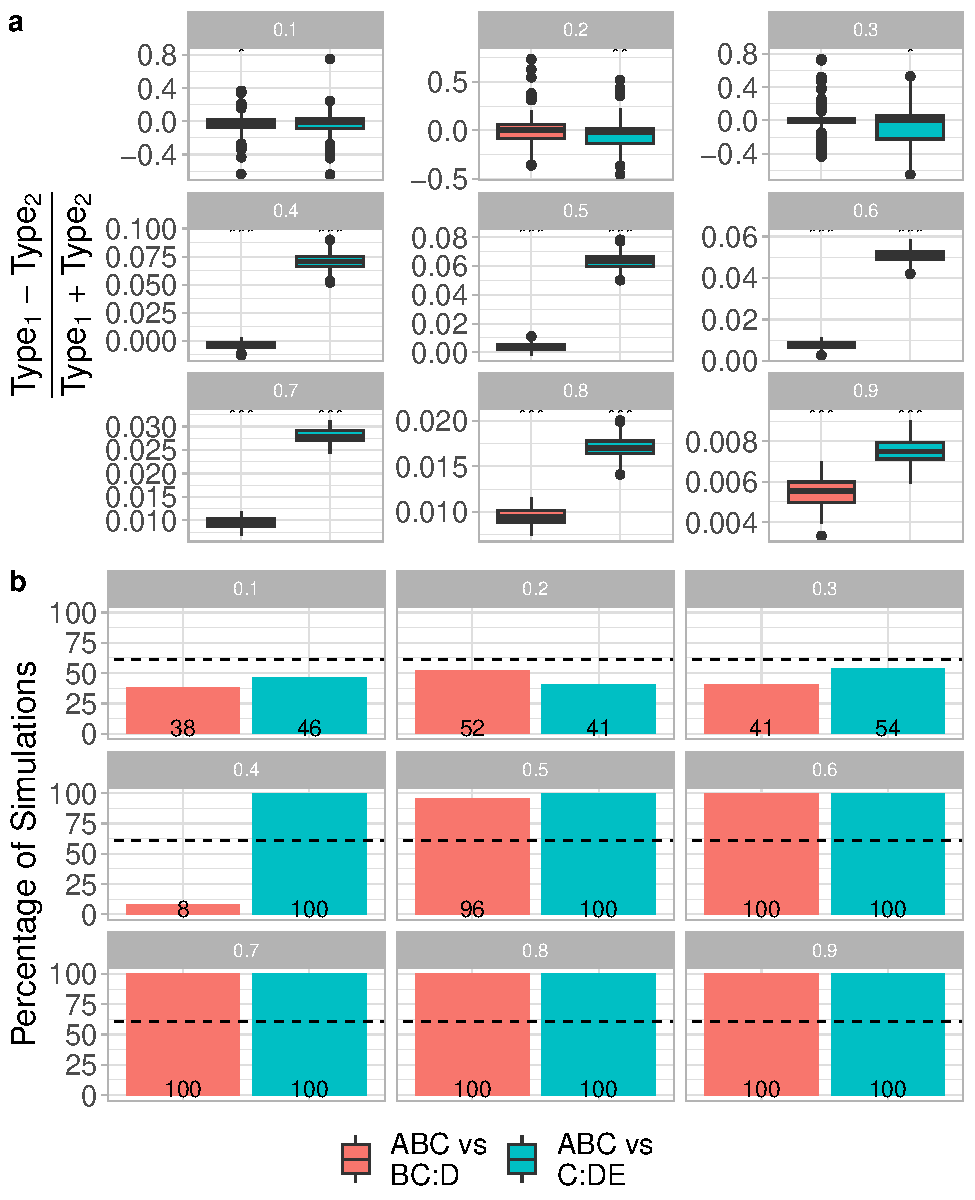
\includegraphics[width=1\linewidth]{tp_model_entrainment_files/figure-latex/basic-experiment-global-create-plot-combined-fw-plot-1} \caption{(a) Difference scores between words and part-words for different forgetting rates (between .1 and .9). The scores are calculated based the global activation as a measure of the network's familiarity with the items. Significance is assessed based on Wilcoxon tests against the chance level of zero. (b). Percentage of simulations with a preference for words for different forgetting rates (between .1 and .9). The simulations are assessed based on the global activation in the network. The dashed line shows the minimum percentage of simulations that is significant based on a binomial test.}\label{fig:basic-experiment-global-create-plot-combined-fw-plot}
\end{figure}

The results are shown in Figure
\ref{fig:basic-experiment-global-create-plot-combined-fw-plot} and Table
\ref{tab:basic-experiment-global-evaluate-diff-print2}. Except for low
forgetting rates of up to .4, the network prefers words over part-words,
with somewhat better performance for words against \emph{C:DE}
part-words, as has been observed in human participants by
\citep{Fiser2002}. In the following, we will thus use forgetting rates
between 0.4 and 0.9 to model the electrophysiological results.

\clearpage

\hypertarget{electrophysiological-results}{%
\subsection{Electrophysiological
results}\label{electrophysiological-results}}

\hypertarget{activation-differences-within-words}{%
\subsubsection{Activation differences within
words}\label{activation-differences-within-words}}

We next asked whether a basic Hebbian learning model can explain
periodic activity found in electrophysiological recordings (XXX),
focusing on the forgetting rates in which the network preferred words to
part-words. In a first analysis, we simply recorded the total network
activation after each syllable in a word has been presented. These
activations were averaged for each syllable position (word-initial,
word-medial and word-final) and for each participant after removing the
first 200 words from the familiarization stream (during which the
network was meant to learn).

As shown in Figure
\ref{fig:basic-experiment-global-print-act-in-words-plot} and Table
\ref{tab:basic-experiment-global-print-act-in-words-table2}, activation
was highest after word-final syllables (though not for very low
forgetting rates for which we did not observe learning in the first
place). As a result, a simple Hebbian learning model can account for
rhythmic activity in electrophysiological recordings with a period
equivalent to the word duration. Critically, however, while previous
electrophysiological responses to statistical structured streams were
interpreted in terms of a response to word onsets (XXX), our results
suggest an alternative interpretation of such results. Rather than
signalling the beginnings and ends of words, an activation maximum after
the third syllable of each word signals the predictability of the third
syllable, while a sudden drop in activation after the first syllable
indicates the lack of predictability.

The reason for which lower forgetting rates do not necessarily lead to
rhythmic activity is the interplay between decay and inhibition. To
assess this possibility, we recorded the number of active neurons after
a burn-in phase of 600 items. As shown in Table
\ref{tab:inspect-number-of-active-neurons-print2} and Figure
\ref{fig:inspect-number-of-active-neurons-plot2}, more neurons remain
active at any point in time when the decay rate is lower, and might thus
inhibit other neurons. When decay limits the effect of residual
inhibitory input from other neurons, the pattern of connections between
neurons then enables the network to exhibit periodic activity.

\begin{figure}
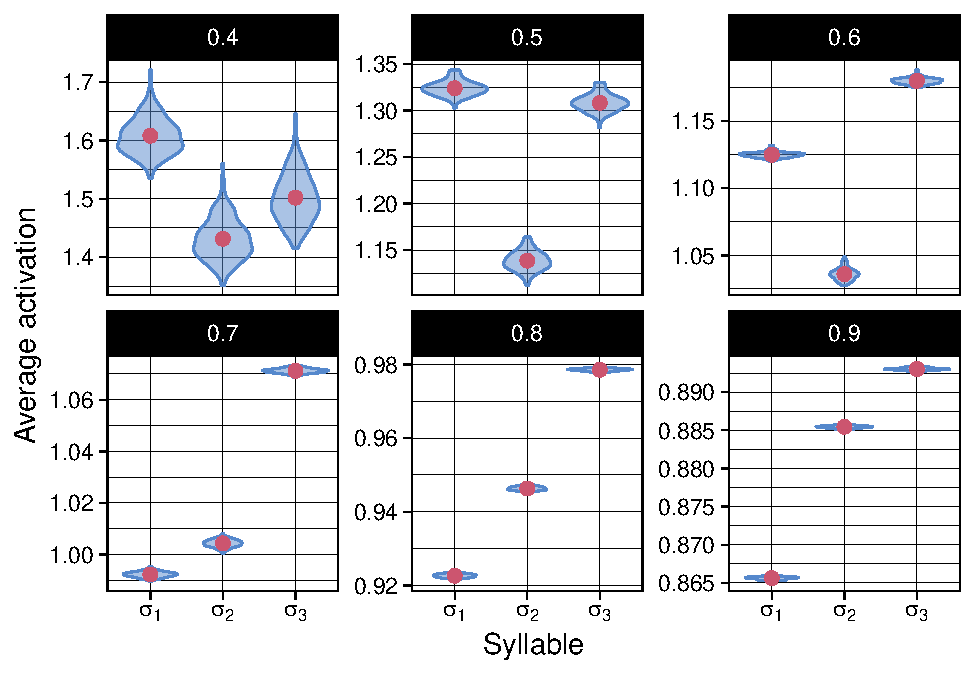
\includegraphics[width=1\linewidth]{tp_model_entrainment_files/figure-latex/basic-experiment-global-print-act-in-words-plot-1} \caption{Average total network activation for different syllables in 100 simulations in Endress and Johnson's network during the familiarization with a stream following Saffran et al. (1996). The facets show different forgetting rates. The results reflect the network behavior after the first 20 presentations of each word. }\label{fig:basic-experiment-global-print-act-in-words-plot}
\end{figure}

\hypertarget{spectral-density}{%
\subsubsection{Spectral density}\label{spectral-density}}

We next analyzed the frequency response of the network to the speech
streams. Specifically, we estimated the spectral density of the time
series corresponding to the total network activation after each time
step (again after a burnin of 200 words), separately for each decay rate
and simulation. We then extracted the frequency with the maximal
density. As shown in Figure
\ref{fig:basic-experiment-global-print-freq-phase-plot}(a), the modal
frequency for decay rates of least .4 was 1/3, corresponding to a period
of three syllables. This results thus suggest again that a simple
Hebbian learning mechanism can entrain to statistical rhythms in the
absence of memory for words.

\hypertarget{phase-analysis}{%
\subsubsection{Phase analysis}\label{phase-analysis}}

Our analyses of the network activations suggest that activations are
strongest for word-final syllables, and that the network entrains to a
periodicity of three syllables. However, the traditional interpretation
of electrophysiological responses to statistical learning is that neural
responses index word-initial syllables. To address this issue more
directly, we calculated the phase of the network activation with respect
to waveforms with maximua on word-initial, word-medial and word-final
syllables, respectively. Specifically, we calculated the cross-spectrum
phase at the winning frequency between the total network activation and
(1) three cosine reference waves with their maxima on the first, second
or third syllable of a word as well as (2) a sawtooth function with its
maximum on the third syllable. As shown in Figure
\ref{fig:basic-experiment-global-print-freq-phase-plot}(b) and Table
\ref{tab:basic-experiment-global-phase-table2}, the activation had a
small relative phase with respect to the cosine with the maximum on the
third syllable or the saw tooth function. In contrast the phase relative
to the cosine with the word-initial maximum was around 120 degrees,
while that with respect to the cosine with the maximum on the second
syllable was around -120 degrees. These spectral analyses thus confirm
that, at least for larger decay rates, the activation increases towards
the end of a word, and that the network activation is roughly in phase
with a function with a maximum on the third syllabe.

\begin{figure}
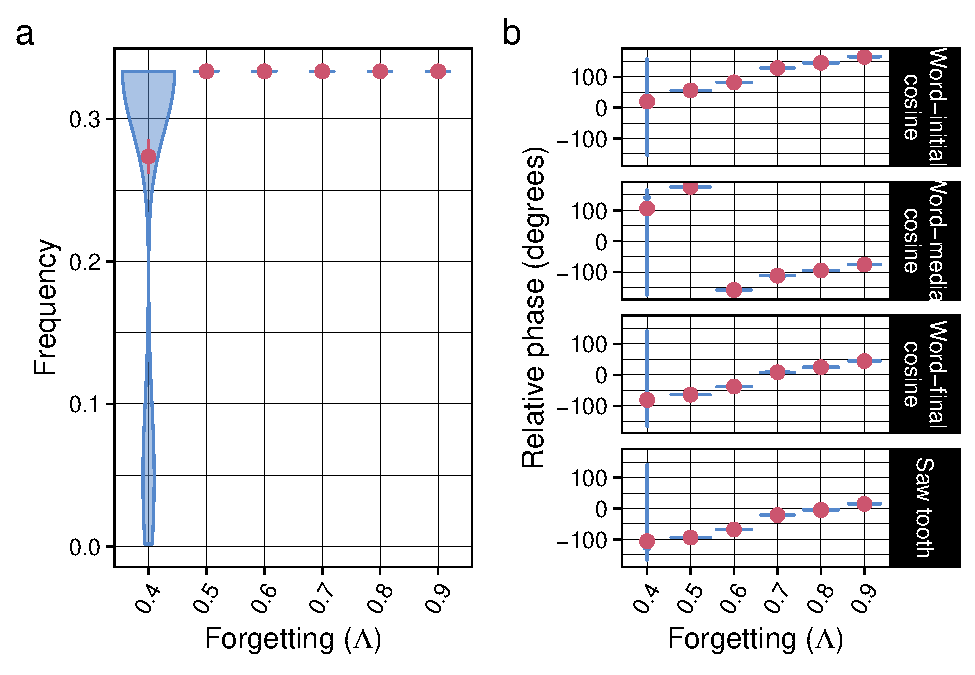
\includegraphics[width=1\linewidth]{tp_model_entrainment_files/figure-latex/basic-experiment-global-print-freq-phase-plot-1} \caption{Spectral analysis of the total network activation in 100 simulations in Endress and Johnson's network during the familiarization with a stream following Saffran et al. (1996). The results reflect the network behavior after the first 20 presentations of each word. (a) Maximal frequency as a function of the forgeting rates. For forgetting rates where learning takes place, the dominant frequency is 1/3, and thus corresponds to the word length. (b) Relative phase (in degrees) at the maximal frequency of the total network activation relative to (from top to bottom) a cosine function with its maximum at word-intial syllables, word-second syllables and word-final syllables and a saw tooth function with the maximum on the third syllable. For forgetting rates where learning takes place, the total activation is in phase with a cosine with its maximum on the word-final syllable as well as with the corresponding saw tooth function.}\label{fig:basic-experiment-global-print-freq-phase-plot}
\end{figure}

\hypertarget{memory-for-word-onsets-vs.-offsets-flo2022}{%
\subsubsection{\texorpdfstring{Memory for word onsets vs.~offsets
\citep{Flo2022}}{Memory for word onsets vs.~offsets {[}@Flo2022{]}}}\label{memory-for-word-onsets-vs.-offsets-flo2022}}

The results so far suggest that a simple Hebbian network can reproduce
rhythmic activity in the absence of memory for words. However,
\citep{Flo2022} suggested that neonates retain at least the first
syllable of statistical defined words. Specifically, they presented
newborns with items starting with two syllables that occurred
word-initially (AB\ldots), and with items starting with a word-medial
syllable (BC\ldots) and observed early ERP differences between these
items.

To reproduce these results, we measured the activation of the network in
response to isolated, bisyllabic \emph{AB} and \emph{BC} test items,
respectively. As shown in Figure
\ref{fig:basic-experiment-global-print-act-after-2syll-plot} and Table
\ref{tab:basic-experiment-global-print-difference-between-parts-of-word2},
the network activation was always greater in response to \emph{BC} items
than to \emph{AB} items except for the largest decay rates. The reasons
is presumably that a \emph{B} syllable is strongly associated with both
\emph{A} and \emph{C} syllables, which are associated with each other in
turn. In contrast, \emph{A} syllables are only strongly associated with
\emph{B} syllables and more weakly with \emph{C} syllables. Upon
presentation of the second syllable, second order activation should thus
be greater for \emph{BC} items than for \emph{AB} items. Be that as it
might, these analyses show that a memory-less system can reproduce
differential responses to \emph{AB} and \emph{BC} items.

\begin{figure}
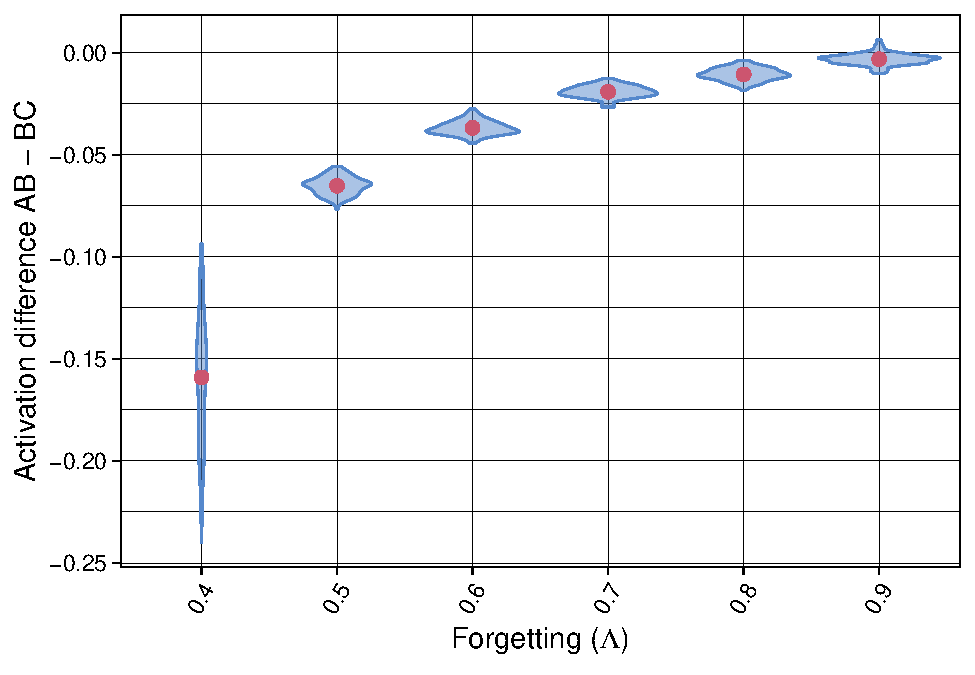
\includegraphics[width=1\linewidth]{tp_model_entrainment_files/figure-latex/basic-experiment-global-print-act-after-2syll-plot-1} \caption{Average difference in the total network activation for the first two syllables of a word (AB) and the first to syllables of a part-word (BC)  in 100 simulations in Endress and Johnson's network after  familiarization with a stream following Saffran et al. (1996). The results reflect the network behavior after the first 20 presentations of each word. Positive values indicate greater activation for the AB items than the BC items.}\label{fig:basic-experiment-global-print-act-after-2syll-plot}
\end{figure}

\clearpage

\hypertarget{discussion}{%
\section{Discussion}\label{discussion}}

To acquire the words of their native language, learners need to extract
them from fluent speech, and might use co-occurrence statistics such as
TPs to do so. If so, high-TP items should be stored in memory for later
use as words. Strong evidence in favor of this possibility comes from
electrophysiology, where rhythmic activity has been observed in response
to statistically structured sequences. In the time domain, different
authors have observed amplitude peaks around the boundaries of
statistically defined words (XXX); in the frequency domain, a frequency
response with a period of the word duration emerges as participants
learn the statistical structure of the speech stream (XXX).

Here, we show that such results can be explained by a simple Hebbian
learning model. When exposed to statistically structure sequences, the
network activation increased towards the end of words due to increased
excitatory input from second order associations. As a result, the
network exhibits rhythmic activations with a period of a word duration.
Critically, given that the network could reproduce these results in the
absence of memory representations for words, earlier
electrophysiological results might thus index the statistical
predictiveness of syllables rather than the acquisition of words. For
example, and as mentioned above, N400 effects observed in statistical
learning tasks (XXX) might not index the onset of words, but rather the
lack of predictibility of word-initial syllables (or the increased
predictibility of word-final syllables). This would also be more
consistent with the initial description of the N400 component as an ERP
component that indexes \emph{unpredictable} events \citep{Kutas2000}.

As mention in the introduction, the view that statistical learning does
not necessarily lead to storage in declarative memory memory is
consistent with long-established dissociations between declarative
memory and implicit learning
\citetext{\citealp{Cohen1980}; \citealp{Finn2016}; \citealp[\citet{Knowlton1996a}]{Graf1984}; \citealp{Poldrack2001}; \citealp{Squire1992}}.
It is also consistent with a variety of behavioral results (see
\citep[\citet{Endress-stat-recall}]{Endress2020} for critical reviews),
including behavioral preferences for unattested high-TP items
\citep{Endress-Action-Axc, Endress-Phantoms-Vision, Endress-Phantoms, Jones2007, Turk-Browne-reversal}),
and the inability of adult learners to repeat back words from
familiarization streams with as few as four
words\citep{Endress-stat-recall}.

In contrast, Statistical Learning might well be important for predicting
events across time
\citep{Endress-stat-recall, Morgan2019, Sherman2020, Turk-Browne2010, Verosky2021}
and space \citep{Theeuwes2022}, an ability that is clearly critical for
mature language processing \citep{Levy2008, Trueswell1999} (as well as
many other processes \citep{Clark2013, Friston2010, Keller2018}). This
suggests the possibility that predictive processing might also be
crucial for word learning, but it is an important topic for further
research to find out how predictive processing interacts with language
acquisition.

\clearpage

\hypertarget{supplementary-information}{%
\section{Supplementary Information}\label{supplementary-information}}

\hypertarget{supplementary-information-1-model-definition}{%
\subsection{Supplementary Information 1: Model
definition}\label{supplementary-information-1-model-definition}}

The activation of the \(i^{th}\) unit is given by

\[
\dot{x_i} = -\lambda_a x_i + \alpha \sum_{j \neq i} w_{ij} F(x_j) - \beta \sum_{j \neq i} F(x_j) + \text{noise}
\]

where \(F(x)\) is some activation function. (Here we use
\(F(x) = \frac{x}{1 + x}\). The first term represents exponential
forgetting with a time constant of \(\lambda_a\), the second term
activation from other units, and the third term inhibition among items
to keep the overall activation in a reasonable range.

The weights \(w_{ij}\) are updated using a Hebbian learning rule

\[
\dot{w}_{ij} = - \lambda_w w_{ij} + \rho F(x_i) F(x_j) 
\]

\(\lambda_w\) is the time constant of forgetting (which we set to zero
in our simulations) while \(\rho\) is the learning rate.

A discrete version of the activation equation is given by

\[
x_i (t+1) = x_i (t) - \lambda_a x_i(t) + \alpha \sum_{j \neq i} w_{ij} F(x_j) - \beta \sum_{j \neq i} F(x_j) + \text{noise}
\]

While the time step is arbitrary in the absence of external input (see
\citep{Endress-Catastrophic-Interference} for a proof), we use the
duration of individual units (e.g., syllables, visual symbols etc.) as
the time unit in our discretization as associative learning is generally
invariant under temporal scaling of the experiment
\citep{Gallistel2000PsychRev, Gallistel2001b}. Further, while only
excitatory connections are tuned by learning in our model, the same
effect could be obtained by tuning inhibition, for example through
tunable disinhibitory interneurons \citep{Letzkus2011}. Here, we simply
focus on the result that a fairly generic network architecture accounts
for the hallmarks of statistical learning that, so far, have eluded
explanation.

The discrete updating rule for the weights is

\[
w_{ij} (t+1) = w_{ij} (t) - \lambda_w w_{ij} (t) + \rho F(x_i) F(x_j) 
\]

Simulation parameters are listed in Table \ref{tab:params}. An \emph{R}
implementation is available at XXX.

\begin{table}

\caption{\label{tab:list-parameters2}\label{tab:params}Parameters used in the simulations}
\centering
\begin{tabular}[t]{ll}
\toprule
Name & Value\\
\midrule
A & 0.7\\
B & 0.4\\
current\_l & 0.9\\
L\_ACT & 0.1, 0.2, 0.3, 0.4, 0.5, 0.6, 0.7, 0.8, 0.9\\
L\_ACT\_DEFAULT & 0.5\\
\addlinespace
L\_ACT\_SAMPLES & 0.1, 0.2, 0.3, 0.4, 0.5, 0.6, 0.7, 0.8, 0.9\\
L\_W & 0\\
N\_ITEMS\_BEFORE\_ACTIVATION\_INSPECTION & 600\\
N\_NEURONS & 19\\
N\_REP\_PER\_WORD & 100\\
\addlinespace
N\_REP\_PER\_WORD\_BURNIN & 50\\
N\_SIM & 100\\
N\_SYLL\_PER\_WORD & 3\\
N\_WORDS & 4\\
NOISE\_SD\_ACT & 0.001\\
\addlinespace
NOISE\_SD\_W & 0\\
R & 0.05\\
\bottomrule
\end{tabular}
\end{table}

\clearpage

\hypertarget{supplementary-information-2-detailed-results}{%
\subsection{Supplementary Information 2: Detailed
results}\label{supplementary-information-2-detailed-results}}

\hypertarget{activation-differences-between-words-and-part-words}{%
\subsubsection{Activation differences between words and
part-words}\label{activation-differences-between-words-and-part-words}}

Table \ref{tab:basic-experiment-global-evaluate-diff-print2} provides
detailed results for the simulations in terms of descriptive statistics
and statistical tests for the simulation testing the recognition of
words and part-words.

\begin{longtable}[t]{llll}
\caption{\label{tab:basic-experiment-global-evaluate-diff-print2}Detailed results for the different forgetting rates and the word vs. part-word comparison (*ABC* vs. *BC:D* and *ABC* vs. *C:DE*), using the global activation as a measure of the network's familiarity with the items. $p_{Wilcoxon}$ represents the *p* value of a Wilcoxon test on the difference scores against the chance level of zero. $P_{Simulations}$ represents the proportion of simulations showing positive difference scores.}\\
\toprule
$\lambda_a$ & Statistic & ABC vs BC:D & ABC vs C:DE\\
\midrule
\endfirsthead
\caption[]{Detailed results for the different forgetting rates and the word vs. part-word comparison (*ABC* vs. *BC:D* and *ABC* vs. *C:DE*), using the global activation as a measure of the network's familiarity with the items. $p_{Wilcoxon}$ represents the *p* value of a Wilcoxon test on the difference scores against the chance level of zero. $P_{Simulations}$ represents the proportion of simulations showing positive difference scores. \textit{(continued)}}\\
\toprule
$\lambda_a$ & Statistic & ABC vs BC:D & ABC vs C:DE\\
\midrule
\endhead

\endfoot
\bottomrule
\endlastfoot
\cellcolor{gray!6}{${100}\times 10^{-3}$} & \cellcolor{gray!6}{{\em M}} & \cellcolor{gray!6}{${-21.8}\times 10^{-3}$} & \cellcolor{gray!6}{${-34.8}\times 10^{-3}$}\\
${100}\times 10^{-3}$ & {\em SE} & ${-2.19}\times 10^{-3}$ & ${-3.50}\times 10^{-3}$\\
\cellcolor{gray!6}{${100}\times 10^{-3}$} & \cellcolor{gray!6}{$p_{Wilcoxon}$} & \cellcolor{gray!6}{${38.0}\times 10^{-3}$} & \cellcolor{gray!6}{${99.2}\times 10^{-3}$}\\
${100}\times 10^{-3}$ & $P_{Simulations}$ & ${380}\times 10^{-3}$ & ${460}\times 10^{-3}$\\
\cellcolor{gray!6}{${200}\times 10^{-3}$} & \cellcolor{gray!6}{{\em M}} & \cellcolor{gray!6}{${15.9}\times 10^{-3}$} & \cellcolor{gray!6}{${-42.9}\times 10^{-3}$}\\
\addlinespace
${200}\times 10^{-3}$ & {\em SE} & ${1.60}\times 10^{-3}$ & ${-4.31}\times 10^{-3}$\\
\cellcolor{gray!6}{${200}\times 10^{-3}$} & \cellcolor{gray!6}{$p_{Wilcoxon}$} & \cellcolor{gray!6}{${881}\times 10^{-3}$} & \cellcolor{gray!6}{${2.44}\times 10^{-3}$}\\
${200}\times 10^{-3}$ & $P_{Simulations}$ & ${520}\times 10^{-3}$ & ${410}\times 10^{-3}$\\
\cellcolor{gray!6}{${300}\times 10^{-3}$} & \cellcolor{gray!6}{{\em M}} & \cellcolor{gray!6}{${26.8}\times 10^{-3}$} & \cellcolor{gray!6}{${-72.6}\times 10^{-3}$}\\
${300}\times 10^{-3}$ & {\em SE} & ${2.69}\times 10^{-3}$ & ${-7.30}\times 10^{-3}$\\
\addlinespace
\cellcolor{gray!6}{${300}\times 10^{-3}$} & \cellcolor{gray!6}{$p_{Wilcoxon}$} & \cellcolor{gray!6}{${595}\times 10^{-3}$} & \cellcolor{gray!6}{${27.4}\times 10^{-3}$}\\
${300}\times 10^{-3}$ & $P_{Simulations}$ & ${410}\times 10^{-3}$ & ${540}\times 10^{-3}$\\
\cellcolor{gray!6}{${400}\times 10^{-3}$} & \cellcolor{gray!6}{{\em M}} & \cellcolor{gray!6}{${-3.86}\times 10^{-3}$} & \cellcolor{gray!6}{${70.8}\times 10^{-3}$}\\
${400}\times 10^{-3}$ & {\em SE} & ${-388}\times 10^{-6}$ & ${7.12}\times 10^{-3}$\\
\cellcolor{gray!6}{${400}\times 10^{-3}$} & \cellcolor{gray!6}{$p_{Wilcoxon}$} & \cellcolor{gray!6}{${305}\times 10^{-18}$} & \cellcolor{gray!6}{${3.96}\times 10^{-18}$}\\
\addlinespace
${400}\times 10^{-3}$ & $P_{Simulations}$ & ${80.0}\times 10^{-3}$ & $1.00$\\
\cellcolor{gray!6}{${500}\times 10^{-3}$} & \cellcolor{gray!6}{{\em M}} & \cellcolor{gray!6}{${3.88}\times 10^{-3}$} & \cellcolor{gray!6}{${63.3}\times 10^{-3}$}\\
${500}\times 10^{-3}$ & {\em SE} & ${390}\times 10^{-6}$ & ${6.37}\times 10^{-3}$\\
\cellcolor{gray!6}{${500}\times 10^{-3}$} & \cellcolor{gray!6}{$p_{Wilcoxon}$} & \cellcolor{gray!6}{${33.8}\times 10^{-18}$} & \cellcolor{gray!6}{${3.96}\times 10^{-18}$}\\
${500}\times 10^{-3}$ & $P_{Simulations}$ & ${960}\times 10^{-3}$ & $1.00$\\
\addlinespace
\cellcolor{gray!6}{${600}\times 10^{-3}$} & \cellcolor{gray!6}{{\em M}} & \cellcolor{gray!6}{${7.56}\times 10^{-3}$} & \cellcolor{gray!6}{${50.7}\times 10^{-3}$}\\
${600}\times 10^{-3}$ & {\em SE} & ${760}\times 10^{-6}$ & ${5.10}\times 10^{-3}$\\
\cellcolor{gray!6}{${600}\times 10^{-3}$} & \cellcolor{gray!6}{$p_{Wilcoxon}$} & \cellcolor{gray!6}{${3.96}\times 10^{-18}$} & \cellcolor{gray!6}{${3.96}\times 10^{-18}$}\\
${600}\times 10^{-3}$ & $P_{Simulations}$ & $1.00$ & $1.00$\\
\cellcolor{gray!6}{${700}\times 10^{-3}$} & \cellcolor{gray!6}{{\em M}} & \cellcolor{gray!6}{${9.45}\times 10^{-3}$} & \cellcolor{gray!6}{${28.0}\times 10^{-3}$}\\
\addlinespace
${700}\times 10^{-3}$ & {\em SE} & ${950}\times 10^{-6}$ & ${2.82}\times 10^{-3}$\\
\cellcolor{gray!6}{${700}\times 10^{-3}$} & \cellcolor{gray!6}{$p_{Wilcoxon}$} & \cellcolor{gray!6}{${3.96}\times 10^{-18}$} & \cellcolor{gray!6}{${3.96}\times 10^{-18}$}\\
${700}\times 10^{-3}$ & $P_{Simulations}$ & $1.00$ & $1.00$\\
\cellcolor{gray!6}{${800}\times 10^{-3}$} & \cellcolor{gray!6}{{\em M}} & \cellcolor{gray!6}{${9.40}\times 10^{-3}$} & \cellcolor{gray!6}{${17.1}\times 10^{-3}$}\\
${800}\times 10^{-3}$ & {\em SE} & ${945}\times 10^{-6}$ & ${1.72}\times 10^{-3}$\\
\addlinespace
\cellcolor{gray!6}{${800}\times 10^{-3}$} & \cellcolor{gray!6}{$p_{Wilcoxon}$} & \cellcolor{gray!6}{${3.96}\times 10^{-18}$} & \cellcolor{gray!6}{${3.96}\times 10^{-18}$}\\
${800}\times 10^{-3}$ & $P_{Simulations}$ & $1.00$ & $1.00$\\
\cellcolor{gray!6}{${900}\times 10^{-3}$} & \cellcolor{gray!6}{{\em M}} & \cellcolor{gray!6}{${5.44}\times 10^{-3}$} & \cellcolor{gray!6}{${7.53}\times 10^{-3}$}\\
${900}\times 10^{-3}$ & {\em SE} & ${547}\times 10^{-6}$ & ${757}\times 10^{-6}$\\
\cellcolor{gray!6}{${900}\times 10^{-3}$} & \cellcolor{gray!6}{$p_{Wilcoxon}$} & \cellcolor{gray!6}{${3.96}\times 10^{-18}$} & \cellcolor{gray!6}{${3.96}\times 10^{-18}$}\\
\addlinespace
${900}\times 10^{-3}$ & $P_{Simulations}$ & $1.00$ & $1.00$\\*
\end{longtable}

\clearpage

\hypertarget{electrophysiological-results-1}{%
\subsubsection{Electrophysiological
results}\label{electrophysiological-results-1}}

\hypertarget{activation-differences-within-words.}{%
\paragraph{Activation differences within
words.}\label{activation-differences-within-words.}}

Table \ref{tab:basic-experiment-global-print-act-in-words-table2} shows
activation differences between pairs of neurons in different positions
within words.

\begin{table}

\caption{\label{tab:basic-experiment-global-print-act-in-words-table2}Difference scores between syllable activations in different positions. P values reflect a Wilcoxon test against the chance level of zero.}
\centering
\begin{tabular}[t]{rrrrrrrrrr}
\toprule
\multicolumn{1}{c}{ } & \multicolumn{3}{c}{$\sigma_2 - \sigma_1$} & \multicolumn{3}{c}{$\sigma_3 - \sigma_2$} & \multicolumn{3}{c}{$\sigma_3 - \sigma_1$} \\
\cmidrule(l{3pt}r{3pt}){2-4} \cmidrule(l{3pt}r{3pt}){5-7} \cmidrule(l{3pt}r{3pt}){8-10}
$\Lambda$ & M & SE & p & M & SE & p & M & SE & p\\
\midrule
0.4 & -0.1767709 & 0.0006546 & 0 & 0.0707578 & 0.0009093 & 0 & -0.1060131 & 0.0013797 & 0\\
0.5 & -0.1853090 & 0.0003695 & 0 & 0.1695923 & 0.0002698 & 0 & -0.0157167 & 0.0001679 & 0\\
0.6 & -0.0889537 & 0.0002555 & 0 & 0.1439090 & 0.0002696 & 0 & 0.0549552 & 0.0000803 & 0\\
0.7 & 0.0120413 & 0.0000504 & 0 & 0.0668421 & 0.0001194 & 0 & 0.0788834 & 0.0000807 & 0\\
0.8 & 0.0237180 & 0.0000243 & 0 & 0.0322516 & 0.0000526 & 0 & 0.0559696 & 0.0000467 & 0\\
\addlinespace
0.9 & 0.0198095 & 0.0000204 & 0 & 0.0075744 & 0.0000249 & 0 & 0.0273839 & 0.0000249 & 0\\
\bottomrule
\end{tabular}
\end{table}

\clearpage

\hypertarget{number-of-active-neurons}{%
\paragraph{Number of active neurons}\label{number-of-active-neurons}}

Table \ref{tab:inspect-number-of-active-neurons-print2} and Figure
\ref{fig:inspect-number-of-active-neurons-plot2} show the number of
simultaneously active neurons as a function of the forgetting rate/

\begin{table}

\caption{\label{tab:inspect-number-of-active-neurons-print2}Number of simultaneously  active neurons as a function of the forgetting rate.}
\centering
\begin{tabular}[t]{rrr}
\toprule
$\Lambda$ & M & SE\\
\midrule
0.1 & 3.897 & 0.061\\
0.2 & 3.991 & 0.029\\
0.3 & 3.612 & 0.006\\
0.4 & 3.200 & 0.002\\
0.5 & 2.995 & 0.001\\
\addlinespace
0.6 & 2.500 & 0.001\\
0.7 & 2.030 & 0.000\\
0.8 & 2.000 & 0.000\\
0.9 & 2.000 & 0.000\\
\bottomrule
\end{tabular}
\end{table}

\begin{figure}
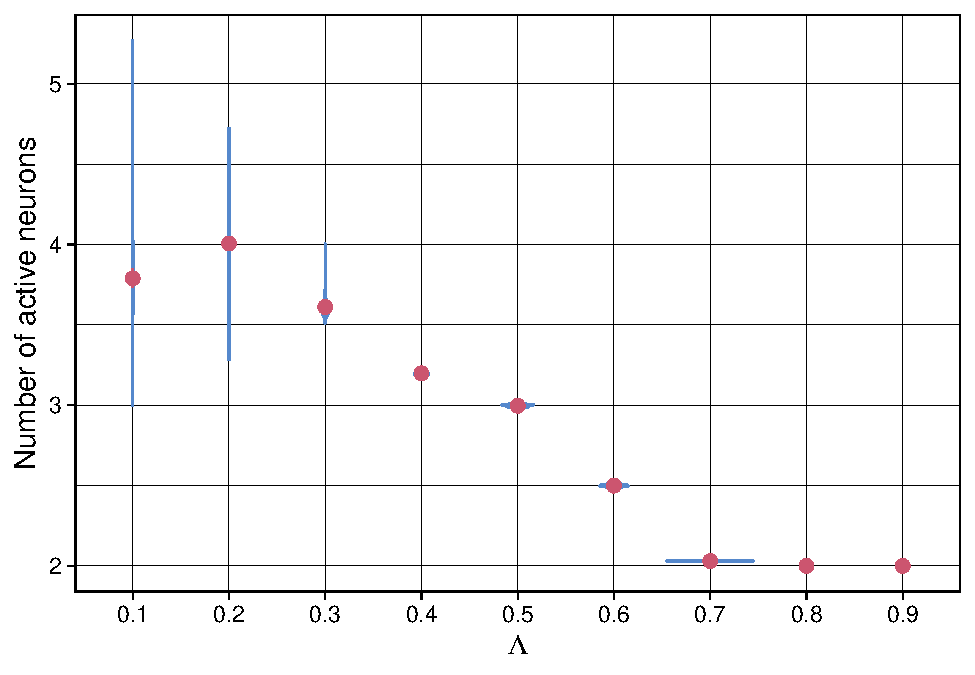
\includegraphics[width=1\linewidth]{tp_model_entrainment_files/figure-latex/inspect-number-of-active-neurons-plot2-1} \caption{Average number of simultaneously active neurons as a function of the forgetting rate.}\label{fig:inspect-number-of-active-neurons-plot2}
\end{figure}

\hypertarget{spectral-density-1}{%
\subsubsection{Spectral density}\label{spectral-density-1}}

\hypertarget{phase-analysis-1}{%
\subsubsection{Phase analysis}\label{phase-analysis-1}}

Table \ref{tab:basic-experiment-global-phase-table2} shows the
descriptives of the relative phase of the network activation relative to
the different syllable positions.

\begin{table}

\caption{\label{tab:basic-experiment-global-phase-table2}Relative phases of the network activation relative to different syllable positions in degrees.}
\centering
\begin{tabular}[t]{rrrrrrrrr}
\toprule
\multicolumn{1}{c}{ } & \multicolumn{8}{c}{Phase in degrees relative to} \\
\cmidrule(l{3pt}r{3pt}){2-9}
\multicolumn{1}{c}{ } & \multicolumn{2}{c}{$\sigma_1$} & \multicolumn{2}{c}{$\sigma_2$} & \multicolumn{2}{c}{$\sigma_3$} & \multicolumn{2}{c}{Saw tooth} \\
\cmidrule(l{3pt}r{3pt}){2-3} \cmidrule(l{3pt}r{3pt}){4-5} \cmidrule(l{3pt}r{3pt}){6-7} \cmidrule(l{3pt}r{3pt}){8-9}
$\Lambda$ & M & SE & M & SE & M & SE & M & SE\\
\midrule
0.4 & 10.65114 & 5.0737440 & 112.03150 & 7.4748326 & -73.557408 & 6.3598153 & -99.853135 & 7.0339273\\
0.5 & 55.72199 & 0.0443242 & 175.72199 & 0.0443242 & -64.278009 & 0.0443242 & -94.278009 & 0.0443242\\
0.6 & 82.00705 & 0.0511961 & -157.99295 & 0.0511961 & -37.992953 & 0.0511961 & -67.992952 & 0.0511961\\
0.7 & 128.41318 & 0.0445116 & -111.58682 & 0.0445116 & 8.413184 & 0.0445116 & -21.586815 & 0.0445116\\
0.8 & 145.04820 & 0.0362621 & -94.95180 & 0.0362621 & 25.048204 & 0.0362621 & -4.951796 & 0.0362621\\
\addlinespace
0.9 & 164.56772 & 0.0473923 & -75.43228 & 0.0473923 & 44.567719 & 0.0473923 & 14.567719 & 0.0473923\\
\bottomrule
\end{tabular}
\end{table}

\clearpage

\hypertarget{memory-for-word-onsets-vs.-offsets}{%
\subsubsection{Memory for word-onsets
vs.~offsets}\label{memory-for-word-onsets-vs.-offsets}}

Table
\ref{tab:basic-experiment-global-print-difference-between-parts-of-word2}
shows the descriptives of activation differences between syllable
bigrams at word onsets and word offsets, respectively.

\begin{table}

\caption{\label{tab:basic-experiment-global-print-difference-between-parts-of-word2}Activation difference between items composed of the first two items of a word and the last two items of a word, when these bigrams were presented in isolation. Positive values indicate greater activation for the AB items than the BC items. The p value reflects a two sided Wilcoxon signed rank test against the chance level of zero}
\centering
\begin{tabular}[t]{rrrr}
\toprule
\multicolumn{1}{c}{ } & \multicolumn{3}{c}{Activation difference between AB and BC items} \\
\cmidrule(l{3pt}r{3pt}){2-4}
$\Lambda$ & M & SE & p\\
\midrule
0.1 & 0.2826406 & 0.7313773 & 0.4280494\\
0.2 & 0.1777287 & 0.4096324 & 0.7322656\\
0.3 & -0.0686097 & 0.0461245 & 0.0002059\\
0.4 & -0.1540030 & 0.0029380 & 0.0000000\\
0.5 & -0.0651579 & 0.0004296 & 0.0000000\\
\addlinespace
0.6 & -0.0368588 & 0.0004031 & 0.0000000\\
0.7 & -0.0193043 & 0.0003164 & 0.0000000\\
0.8 & -0.0101854 & 0.0002769 & 0.0000000\\
0.9 & -0.0028198 & 0.0002854 & 0.0000000\\
\bottomrule
\end{tabular}
\end{table}

  \bibliography{../misc/ansgar.bib}

\end{document}
